\documentclass[letter,8pt,landscape]{article}
\usepackage{fontspec}
\usepackage[T1]{fontenc}
\usepackage[frenchb]{babel} 
\usepackage{amssymb,amsmath,amsthm,amsfonts}
\usepackage{multicol,multirow}
\usepackage{calc}
\usepackage{graphicx}
\usepackage{ifthen}
\usepackage[landscape]{geometry}
\usepackage[colorlinks=true,citecolor=blue,linkcolor=blue]{hyperref}


\ifthenelse{\lengthtest { \paperwidth = 11in}}
    { \geometry{top=.1in,left=.1in,right=.1in,bottom=.1in} }
	{\ifthenelse{ \lengthtest{ \paperwidth = 297mm}}
		{\geometry{top=1cm,left=1cm,right=1cm,bottom=1cm} }
		{\geometry{top=1cm,left=1cm,right=1cm,bottom=1cm} }
	}
\pagestyle{empty}
\makeatletter
\renewcommand{\section}{\@startsection{section}{1}{0mm}%
                                {-1ex plus -.5ex minus -.2ex}%
                                {0.5ex plus .2ex}%x
                                {\normalfont\large\bfseries}}
\renewcommand{\subsection}{\@startsection{subsection}{2}{0mm}%
                                {-1explus -.5ex minus -.2ex}%
                                {0.5ex plus .2ex}%
                                {\normalfont\normalsize\bfseries}}
\renewcommand{\subsubsection}{\@startsection{subsubsection}{3}{0mm}%
                                {-1ex plus -.5ex minus -.2ex}%
                                {1ex plus .2ex}%
                                {\normalfont\small\bfseries}}
\makeatother
\setcounter{secnumdepth}{0}
\setlength{\parindent}{0pt}
\setlength{\parskip}{0pt plus 0.5ex}
% -----------------------------------------------------------------------

\begin{document}

\raggedright
\footnotesize

\begin{multicols}{3}
\setlength{\premulticols}{1pt}
\setlength{\postmulticols}{1pt}
\setlength{\multicolsep}{1pt}
\setlength{\columnsep}{2pt}

\vfill
\smallskip

  \section{General Concepts}
  Amdahl's law: $\text{overall speedup} = \frac{1}{(1-p) +
  \frac{p}{N}}$

  Gustafson's Law - Weak Scaling: $S = (1-p) + p \times N$

  Note that $N$: nproc and $p$: proportion of parallel code. Gustafson's Law
  addresses fixed problem size of Amdahl's law and instead gives the theoretical
  speedup a task gains from being parallelized. predacated that serial code in a
  parallelized environment remains fixed as problem scales as such assumes that
  problem scales with number of workers. Countering of serial component by
  increasing volume of computation. Amdahl's law is predicated under the strong
  scaling model where the problem size remains fixed.

  Little's Law: $L = p \times \lambda$
  
  Based on the idea of how to saturate compute volume. hid latency while
  performing other things during wait eg. memory access or pipeline stall.

  $\text{Memory instructions} = \text{memory}_\text{bw} \times \text{memory}_\text{latency}$

  $\text{Arithmetic Instructions} = \text{arith}_\text{throughput} \times \text{arith}_\text{latency}$

  $\text{Concurrency} = \text{memory}_\text{bandwidth} \times \text{memory}_\text{latency}$

  \subsection{Speedup \& Efficiency}

  GPU speedup: $S_\text{GPU} = \frac{\text{fastest CPU completion
  time}}{\text{completion time on GPU}}$

  Parallel Compute speedup: $S_p = \frac{\text{single threaded
  completion}}{\text{parallel completion}}$

  Efficiency: $E_p = \frac{S_p}{p}$ where $p$: nproc


  Scaled Speedup: $PT_p = T_1 + T_o$, where $T_1$ is serial runtime and $T_o$ is
  parallel overhead.

  Isoefficiency: There is some function $f(P) = N$ that specifies the problem
  size ($N$) that keeps parallel efficiency constant. given that efficiency is
  given as $E = \frac{S}{P} = \frac{1}{1 + \frac{T_o}{T_1}} = \frac{1}{1 +
  \frac{T_o}{Wt_c}} $ with $T_1 = Wt_c$ where $W$: problem size in operations
  and $t_c$: time per op. we note that $T_o$ is a function of $P$ as such $W$
  should grow as a function of $P$ as well. eg. with Fat tree topology $T_o =
  O(\log(P))$ -- network diameter

  \subsubsection{Performance Prediction}
  Computation time: $T_\text{comp} = D(n) + \frac{W(n) - D(n)}{p}$, where $W(n)$
  is the number of work nodes and $D(n)$ is nodes on critical path. Ratio
  implies how parallelizability it is $\frac{W(n)}{D(n)}$. eg, Matrix multiply
  -- $W(n) = n$: number of multiplies -- $D(n) = \log(n)$: reduction add. Ratio
  shows massive potential for parallelization

  Compute time: $T(1, (m,n)) =$ time for best serial algorithm on a $m\times n$
  problem. $T(p, (m,n)) = T(1,(m,n)) + T_\text{comm}$: runtime on $p$ processes
  where $(m,n) = \frac{N}{(p,q)}$ with $p\times q$ being process grid on
  $N\times N$ problem.
  $T_\gamma(p, (m,n)) = \frac{T(P,(m,n))}{m\cdot n\cdot \text{N iterations}}$.
  
  Grind time: parallel performance ignoring communication time
  $T_\text{comm}$



  \subsubsection{Super Linear Speedup}
  when $S_p > P \implies \frac{S_p}{p} = E_p > 1$. Real super linear scaling
  exiss when $P$ scales things such as memory/cache sizes/bandwidth or yields
  more network bandwidht. Can be faked with poor algorithm or measurement
  technique. often suggests a better serial algorithm exists since $S_p =
  \frac{T_s}{T_p}; E_p = \frac{S_p}{p} > 1 \implies T_s > p\times T_p$ meaning
  $T_s$ is not optimal and there exists some serial that could perform the
  parallel component and take less time than original.


  \subsection{Roofline Model}
  Peak performance for each processor is intrinsic based on clock speed with
  bandwidth determining how steep the slop is. $q = \frac{\text{Flops}}{\text{Bytes}}$.
  Where "bytes" is amount of memory operations and flops being the computation
  amount.
  \begin{center}
    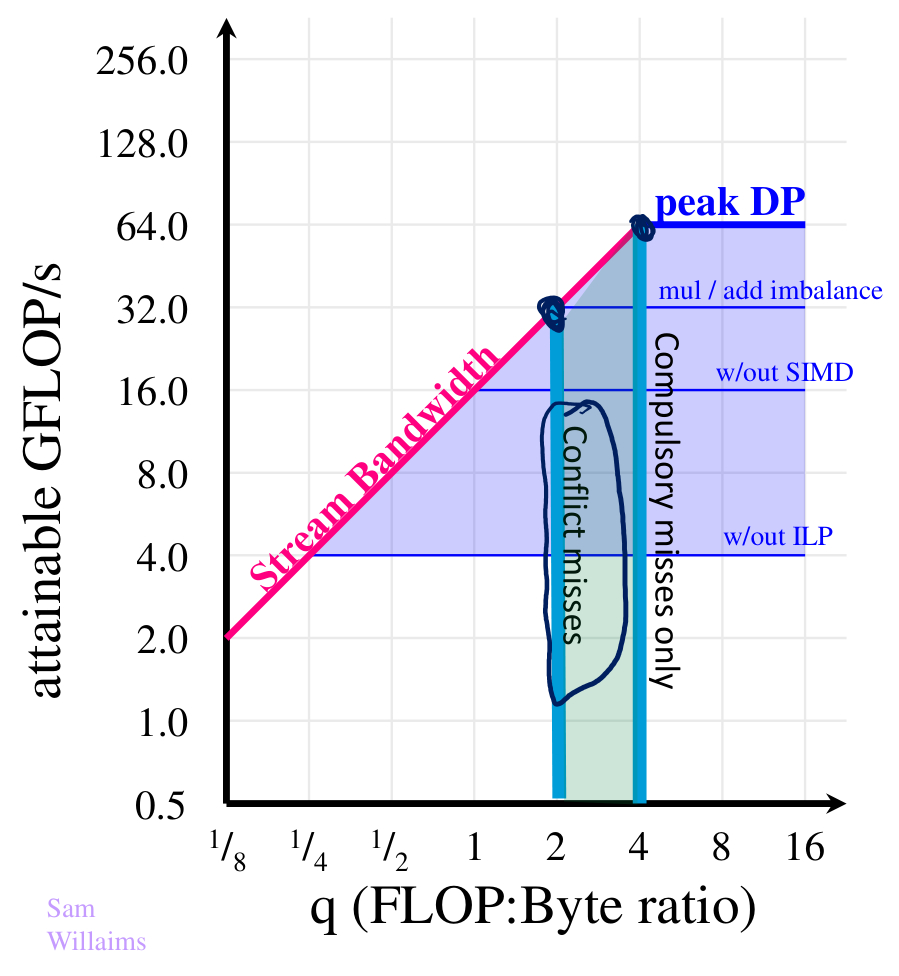
\includegraphics[width=1.5in]{images/roofline-eg.jpg}
  \end{center}
  

  \subsection{Memory Hierarchy}

  Layers of cache hierarchy are to tradeoff access speed and capacity.

  \begin{center}
    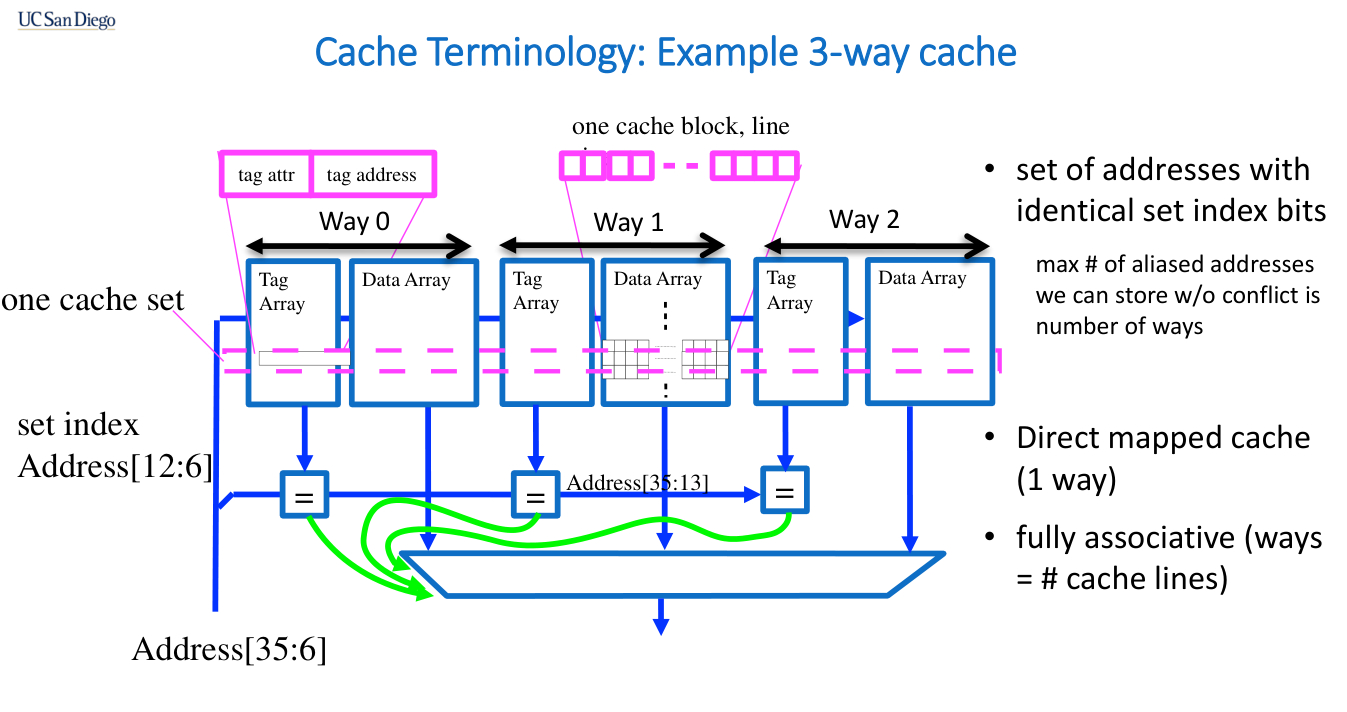
\includegraphics[width=\linewidth]{images/nway-cache.jpg}
  \end{center}
  3-way cache extends to $n$-way cache

  Cold miss: miss due to first access of data

  Capacity miss: miss due to cache being full

  Conflict miss: miss due to too many set aliases for memory addresses mapping
  to caches

  Temporal Cache locality: recent use of memory address

  Spatial Cache locality: use of a memory address is close to a previously used
  one

  \section{Matrix Multiply}
  Naive Matrix Mult: $q = \frac{2n^3}{n^3 + 3n^2}$. With $2n^3$: $n^3$ being
  iterating over elements of $A,B$ and $2$ from add and mult. $n^3$ comes from
  loading blocks of $B$ (hot loop), $n^2$ comes from loading blocks of $A$ and
  load and store to blocks of $C$.

  Blocking Matrix Mult: Same comp intensity as the naive just access pattern is
  more cache friendly. So performance ends up being some scalar fraction of
  Naive as $N$ increases.

  GOTOblas:
  \begin{center}
    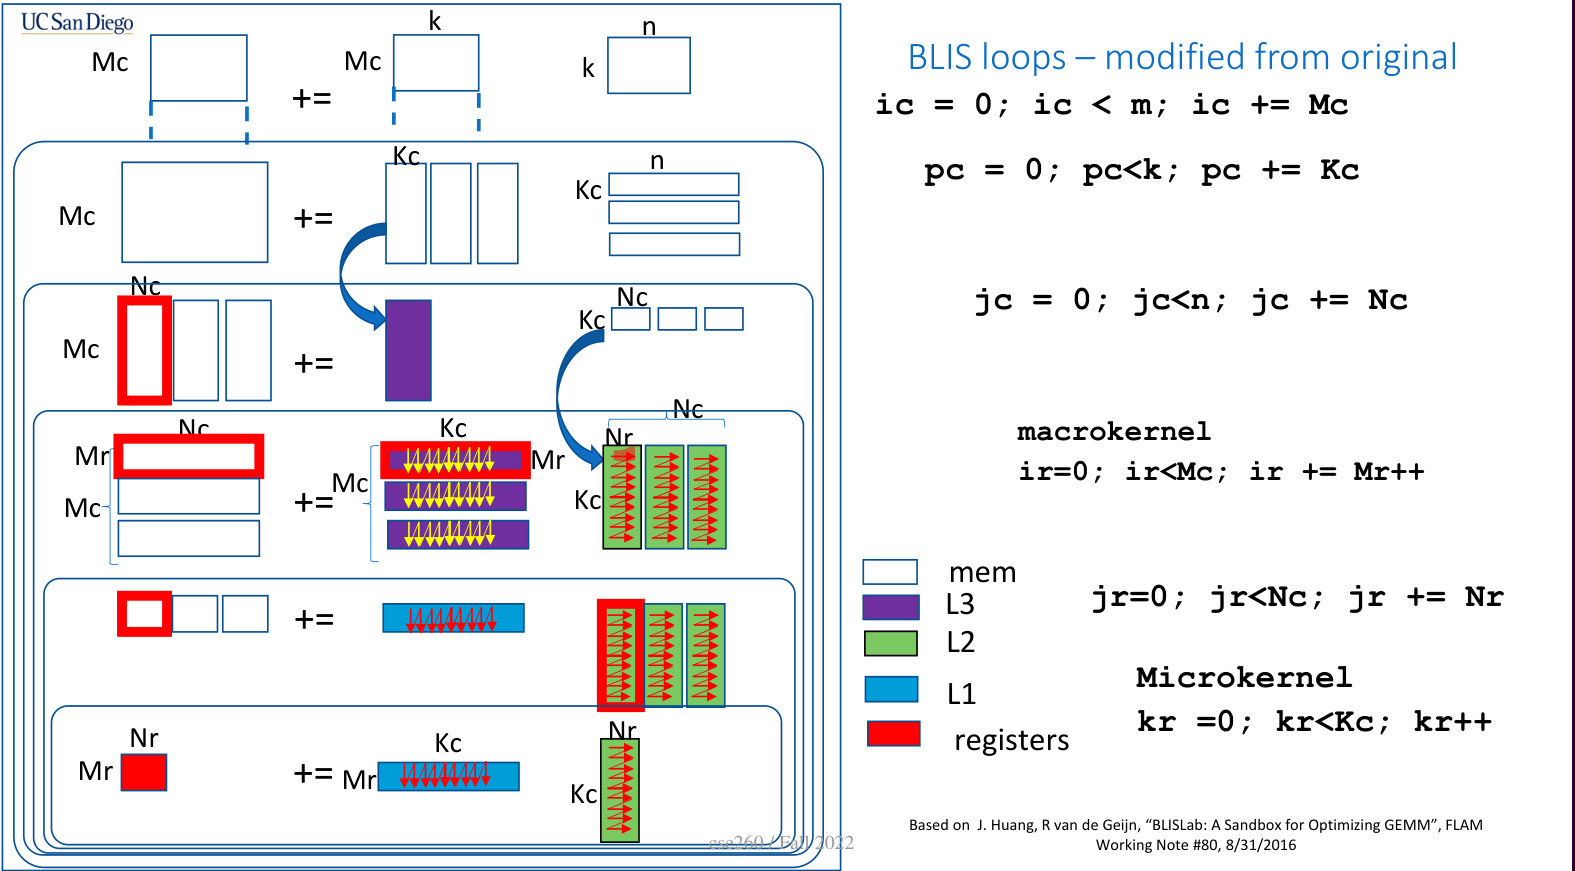
\includegraphics[width=\linewidth]{images/gotoblas.jpg}
  \end{center}
  $q = \frac{2n^3}{(2N + 2) * \frac{n^2}{L}}$. Where $N$ is size of matrix macro
  kernel and $L$ is size of cache line.

  \subsection{Parallel Matrix Multiply}

  \section{SIMD}

  \section{Multithreading}

  \section{Gpu Architecture}

  \section{Message Passing}

  \subsection{MPI Perf modeling}

  \subsection{Communication Parameters}

  \section{Asics}

  \section{Higher Level Abstractions}

  \section{Examples}
  





\end{multicols}

\end{document}

